\begin{bibunit}[apalike]
\begin{frame}%[label=frm:20]
    \frametitle{Estabilidad en Media Cuadrática \cite{saito1996stability}}
	\biblio{BibliografiaTesis}
\end{frame}
\end{bibunit}
%%%%%%%%%%%%%%%%%%%%%%%%%%%%%%%%%%%%%%%%%%%%%%%%%%%%%%%%%%%%%%%%%%%
\begin{frame}%[label=frm:20]
	\frametitle{Estabilidad en Media Cuadrática}
	\begin{overlayarea}{\textwidth}{.25\textheight}	
		\only<1-4>{
			\begin{empheq}[box=\shadowbox*]{equation*}
				dy(t)=\lambda y(t) dt +\beta dW_t, \quad y_0=cte, \lambda, \beta \in
				\mathbb{C} \qquad \tag{(DP)}
			\end{empheq}
		}
		\only<5>{
		 	\begin{empheq}[box=\shadowbox*]{equation*}
				\lim_{t \to \infty}\mathbb{E}[|y(t)|^2]=-\frac{|\beta|^2}{2Re(\lambda)}.
			\end{empheq}	
		}	
	\end{overlayarea}
	\begin{columns}	
		\column{.5\textwidth}		
		\begin{overlayarea}{\textwidth}{\textheight}				
			\centering{Euler-Mayurama}		
			\only<1->{				
				\begin{empheq}[box={\ovalbox}]{align*}
						Y_{n+1} = &(1+\lambda h) Y_n +\beta \Delta W_n 
				\end{empheq}							
			}

		\only<2->{
			Si $Re(\lambda h)<0$			
			\begin{align*}
  					\mathbb{E}[|Y_{n+1}|^2]
  					\xrightarrow{n\to\infty}  			
  					\colorbox{darkyellow}{
  				 		$\frac{-|\beta|^2 }{2Re(\lambda)+|\lambda|^2h}$
  					}
  				\end{align*}
		}
		\end{overlayarea}
%--------------------------------------------------------------------------------		
		\column{.6\textwidth}		
		\begin{overlayarea}{\textwidth}{\textheight}	
			\only<3->{
				\centering{\alert<5->{\textbf{Steklov}}}					
					\begin{empheq}[box=\mybluebox]{align*}
						Y_{n+1} = & Y_n \exp(\lambda h)+\beta \Delta W_n
					\end{empheq}
			}						
			\only<4->{
				Si $Re(\lambda)<0$
				\begin{align*}
  					\mathbb{E}[|Y_{n+1}|^2]
  					\xrightarrow{n\to\infty}
  					\colorbox{hellcyan}{
  				 		$\frac{-|\beta|^2 h}{\exp(2Re(\lambda)h)-1}$
  					}
  				\end{align*}		
			}
		\end{overlayarea}
	\end{columns}
	%\biblio{BibliografiaTesis}
\end{frame}
%\end{bibunit}
%%%%%%%%%%%%%%%%%%%%%%%%%%%%%%%%%%%%%%%%%%%%%%%%%%%%%%%%%%%%%%%%%%%%%%%%%%%%%%%%%%%%%%%%%%%%%%%%%
\begin{frame}
  \frametitle{Estabilidad en Media Cuadrática}
  \begin{empheq}{equation}
 		dy(t)=\lambda y(t) dt +\beta dW_t, \qquad y_0=cte., \lambda, \beta \in \mathbb{C} \tag{E}.
  \end{empheq}
   \begin{columns}
	  \column{.55\textwidth}
		\begin{definicion}[Consistencia lineal en MC]
	 		Un esquema numérico para  la ecuación (E) se dice 
	 		\textcolor{red}{
		 		asintóticamente consistente en media
		 		cuadrática
	 		}
		 	 si la solución numérica satisface
 		$$
 		  \lim_{\substack{ n\to \infty\\ h\to 0}} y_n= \frac{-\beta}{2Re(\lambda)}.
 		$$
 	  \end{definicion}
	  \column{.5\textwidth}
 	  \begin{Teorema}
 		 El esquema Steklov para la ecuación (E), es 
 		 \textcolor{red}{asintóticamente consistente en MC.}
 	  \end{Teorema}
  \end{columns}
\end{frame}
%%%%%%%%%%%%%%%%%%%%%%%%%%%%%%%%%%%%%%%%%%%%%%%%%%%%%%%%%%%%%%%%%%%%%%%%%%%%%%%%%%%%%%%%%%%%%%%%%
\begin{frame}
	\frametitle{Estabilidad lineal por trayectorias}
	\begin{empheq}{equation*}
		dy(t)=\lambda y(t) dt +\beta dW_t, \qquad y_0=cte., \lambda, \beta \in \mathbb{R} \tag{E}.
	\end{empheq}
	\begin{columns}
		\column{.5\textwidth}
			\begin{overlayarea}{\textwidth}{.5\textheight}
				\centering Pullback attractor
				\only<2->{
					\begin{empheq}[box=\shadowbox*]{equation*}
						\lim_{t_0\to-\infty} y(t) =\widehat{O}_t %
						:= e^{\lambda t}\int\limits_{-\infty}^{t}e^{-\lambda s}dW_s, 
					\end{empheq}
				}
		\end{overlayarea}
		\column{.5\textwidth}
			\begin{overlayarea}{\textwidth}{.5\textheight}
			\vspace{-1.0cm}
			\only<3->{
				\begin{Teorema}
					Sea $\lambda<0$,  el método Steklov para (E)
					tiene el siguiente atractor
					\begin{equation*}
						\widehat{O}_n^{(h)}  :=
						\xi \sum_{j=-\infty}^{n-1}\exp(\lambda h(n-1-j)) \Delta B_j,
					\end{equation*}
					$\widehat{O}_n^{(h)} \to \widehat{O}_t$, \quad $h\to 0$, \quad pathwise.
				\end{Teorema}
			}
			\end{overlayarea}
	\end{columns}
	\begin{bibunit}[alpha]
		\nocite{Buckwar2011a}
		\biblio{BibliografiaTesis}
	\end{bibunit}		
\end{frame}
%%%%%%%%%%%%%%%%%%%%%%%%%%%%%%%%%%%%%%%%%%%%%%%%%%%%%%%%%%%%%%%%%%%%%%%%%%%%%%%%%%%%%%%%%%%%%%%%%
\begin{frame}
	\frametitle{Estabilidad en Media Cuadrática Ruido Multiplicativo}
	\begin{empheq}[box=\shadowbox*]{equation*}
		dy(t)=\lambda y(t) dt +\xi y(t) dW_t, \qquad y_0=cte., 
		\ \lambda, \xi \in \mathbb{R} \tag{E}.
	\end{empheq}
		\begin{columns}
			\column{.3\textwidth}
				\begin{overlayarea}{\textwidth}{\textheight}
					\only<2->{
						\begin{exampleblock}{MS-estabilidad Lineal}
							\begin{itemize}
								\item
								diagonal (EM)
								\item
								vertical (Steklov)
								\end{itemize}
						\end{exampleblock}
					}
				\end{overlayarea}
			\column{.7\textwidth}
				\begin{overlayarea}{\textwidth}{\textheight}
					\only<3->{
						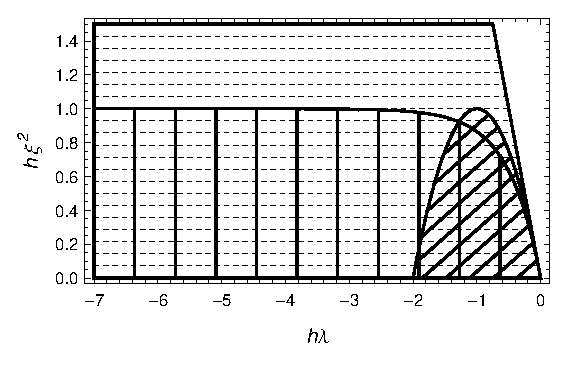
\includegraphics[width=1\linewidth]{images/StabilityPlotMultiplicativeNoise}
					}
				\end{overlayarea}
		\end{columns}
\end{frame}



